\section{Graph Partitioning with Demands on Trees}\label{sec:tree-configuration-lp}

For the special case of the \textsc{Graph Partitioning with Demands} problem where the supply graph is a tree, one could ask whether the problem is polynomial-time or pseudo-polynomial-time solvable.
We answer this question in the negative below by showing inapproximability (and also strong NP-hardness) even on stars.
We then ask whether one can improve the approximation guarantee given by Theorem \ref{thm:gpd-extension}, since the constant provided by that theorem is relatively large.
We give three polynomial-time bicriteria approaches for arbitrary demand weights: anchored-LP rounding, centroid recursion based on submodular maximum coverage, and a hybrid combining anchored-LP normalization with centroid recursion. Each approach has an approximation guarantee depending on $\rho$ and $\eta$, so the best method can vary across parameter ranges.
Taking the best of their guarantees gives approximation ratios depending on $\rho$ and $\eta$ that improve on the constant provided by Theorem~\ref{thm:gpd-extension}. As a corollary, we obtain a polynomial-time $\frac{4e}{e-1}$-approximation for \textsc{Hierarchical Clustering with Demands} on trees.

We write $\OPT_{B_\rho}(T)=\OPTdem{T}{\rho}$ for the minimum cost of a partition whose components have internal demand at most $B_\rho$.

\subsection{Hardness on stars}

The following statement shows an approximation-preserving reduction from the \textsc{Vertex Cover} problem. The reduction is very simple.

\begin{theorem}\label{thm:tree-gpd-vertex-cover-hardness}
    For every fixed rational $\rho\in(0,1)$, \textsc{Graph Partitioning with Demands} is as hard to approximate as \textsc{Vertex Cover}, even when the supply graph is a star.
\end{theorem}
\begin{proof}
    Let $G=(U,F)$ be a \textsc{Vertex Cover} instance. Let $V=U\cup\{r,d\}$. Construct a supply star $E$ with center $r$, leaves $U$, and one additional leaf $d$. Set $c(rd)=\infty$ and $c(ru)=1$ for every $u\in U$. The edges of the demand graph are $F\cup\{rd\}$ where $w\br{rd}=\frac{\rho \cdot \spr{F}}{1-\rho}$ and, for every $uv\in F$, $w\br{uv}=1$. If necessary, multiply all demand weights by a common denominator to make them integral.

    The total demand is $W=w\br{rd}+\spr{F}$, and hence $\rho \cdot W=w\br{rd}$. Any solution of cost at most $\spr{U}$ leaves $rd$ uncut, otherwise its cost becomes $\infty$. For any solution $C$, let $H\in T\setminus C$ be the component containing $r$. If $H$ contained both endpoints of some edge $uv\in F$, its internal demand would exceed $w\br{rd}$. Therefore, the set $C_H=V\setminus V\br{H}$ forms a vertex cover. Moreover, we have that $c\br{C}=\spr{C_H}$ which means that the cost of any solution for the \textsc{Graph Partitioning with Demands} instance equals the size of some vertex cover. Conversely, any cover $C_H\subseteq U$ gives rise to a solution $C$ by cutting all edges incident to $C_H$, which has cost $\spr{C_H}$. Thus the reduction preserves approximation ratios.
\end{proof}

Combining Theorem~\ref{thm:tree-gpd-vertex-cover-hardness} with the known hardness of \textsc{Vertex Cover} gives the following consequence.
\begin{corollary}\label{cor:tree-gpd-hardness}
    For every $\varepsilon>0$, \textsc{Graph Partitioning with Demands} on stars is hard to approximate within $\sqrt{2}-\varepsilon$ unless $P=NP$, and within $2-\varepsilon$ assuming the Unique Games Conjecture~\cite{TowardsAProofOfThe2To1GamesConjecture,VertexCoverMightBeHardToApproximateToWithin2MinusEpsilon}.
\end{corollary}


\subsection{Anchor-LP-based algorithm}

Our first algorithm is based on an anchored linear programming relaxation of the problem. The idea is that for each vertex $a\in V$, which we call an \emph{anchor}, we would like to have a constraint upper bounding the internal demand of the component containing $a$. To do this, our LP consists of two kinds of variables, the ones corresponding to the edges that are cut (the $x_e$ variables) and the ones denoting whether a given demand edge is internal to the component anchored at $a$ (the $z^a_{uv}$ variables).
After solving the LP, we pick an arbitrary global root $r\in V$ and we calculate the distance $\dist(u)=\dist_x(r,u)$ of every vertex $u\in V$ from the root. This step can be seen as projecting the vertices of the tree onto the real line where $r$ lays at the origin and the position of each vertex $u$ is given by $\dist_x(r,u)$. Then, we pick an apropriate number $R$ and subdivide the line into intervals of length $R$. Whenever a given edge crosses an interval boundary, we cut it in the solution. However, in order for this approach to work, we draw a random phase $\theta\in[0,R)$ and shift all intervals by this value $\theta$. This randomized rounding gives a solution with low cost in expectation and can be derandomized by trying all possible relevant phases. Figure~\ref{fig:anchored-lp-threshold-line} illustrates the embedding and threshold locations.

\begin{figure}[!tbp]
  \centering
  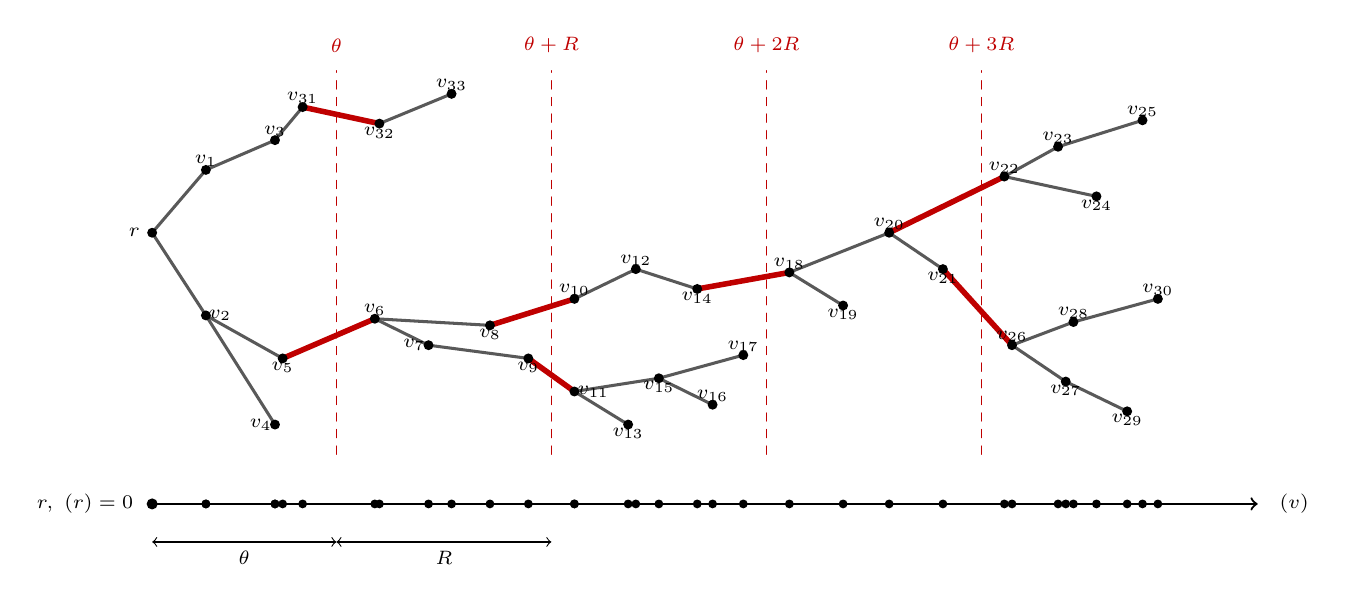
\begin{tikzpicture}[
    x=1.95cm,
    y=0.42cm,
    line cap=round,
    line join=round,
    treeedge/.style={draw=black!65,line width=1.1pt},
    cutedge/.style={draw=red!75!black,line width=2pt}
  ]
    % Horizontal position is D(v); vertical position gives a clean tree layout.
    \coordinate (rT) at (0,0);
    \coordinate (v1T) at (0.35,1.9);
    \coordinate (v2T) at (0.35,-2.5);
    \coordinate (v3T) at (0.8,2.8);
    \coordinate (v4T) at (0.8,-5.8);
    \coordinate (v5T) at (0.85,-3.8);
    \coordinate (v6T) at (1.45,-2.6);
    \coordinate (v7T) at (1.8,-3.4);
    \coordinate (v8T) at (2.2,-2.8);
    \coordinate (v9T) at (2.45,-3.8);
    \coordinate (v10T) at (2.75,-2.0);
    \coordinate (v11T) at (2.75,-4.8);
    \coordinate (v12T) at (3.15,-1.1);
    \coordinate (v13T) at (3.1,-5.8);
    \coordinate (v14T) at (3.55,-1.7);
    \coordinate (v15T) at (3.3,-4.4);
    \coordinate (v16T) at (3.65,-5.2);
    \coordinate (v17T) at (3.85,-3.7);
    \coordinate (v18T) at (4.15,-1.2);
    \coordinate (v19T) at (4.5,-2.2);
    \coordinate (v20T) at (4.8,0.0);
    \coordinate (v21T) at (5.15,-1.1);
    \coordinate (v22T) at (5.55,1.7);
    \coordinate (v23T) at (5.9,2.6);
    \coordinate (v24T) at (6.15,1.1);
    \coordinate (v25T) at (6.45,3.4);
    \coordinate (v26T) at (5.6,-3.4);
    \coordinate (v27T) at (5.95,-4.5);
    \coordinate (v28T) at (6.0,-2.7);
    \coordinate (v29T) at (6.35,-5.4);
    \coordinate (v30T) at (6.55,-2.0);
    \coordinate (v31T) at (0.98,3.8);
    \coordinate (v32T) at (1.48,3.3);
    \coordinate (v33T) at (1.95,4.2);

    % Four thresholds t_k = theta + k R, k=0,...,3.
    \foreach \x in {1.2,2.6,4.0,5.4} {
      \draw[red!75!black,dashed,thin] (\x,-6.7) -- (\x,4.9);
    }

    % The four thresholds cross 2, 2, 1, and 2 edges, respectively.
    \draw[treeedge] (rT) -- (v1T);
    \draw[treeedge] (rT) -- (v2T);
    \draw[treeedge] (v1T) -- (v3T);
    \draw[treeedge] (v3T) -- (v31T);
    \draw[cutedge] (v31T) -- (v32T);
    \draw[treeedge] (v32T) -- (v33T);
    \draw[treeedge] (v2T) -- (v4T);
    \draw[treeedge] (v2T) -- (v5T);
    \draw[cutedge] (v5T) -- (v6T);
    \draw[treeedge] (v6T) -- (v7T);
    \draw[treeedge] (v6T) -- (v8T);
    \draw[treeedge] (v7T) -- (v9T);
    \draw[cutedge] (v8T) -- (v10T);
    \draw[cutedge] (v9T) -- (v11T);
    \draw[treeedge] (v10T) -- (v12T);
    \draw[treeedge] (v12T) -- (v14T);
    \draw[treeedge] (v11T) -- (v13T);
    \draw[treeedge] (v11T) -- (v15T);
    \draw[treeedge] (v15T) -- (v16T);
    \draw[treeedge] (v15T) -- (v17T);
    \draw[cutedge] (v14T) -- (v18T);
    \draw[treeedge] (v18T) -- (v19T);
    \draw[treeedge] (v18T) -- (v20T);
    \draw[treeedge] (v20T) -- (v21T);
    \draw[cutedge] (v20T) -- (v22T);
    \draw[cutedge] (v21T) -- (v26T);
    \draw[treeedge] (v22T) -- (v23T);
    \draw[treeedge] (v22T) -- (v24T);
    \draw[treeedge] (v23T) -- (v25T);
    \draw[treeedge] (v26T) -- (v27T);
    \draw[treeedge] (v26T) -- (v28T);
    \draw[treeedge] (v27T) -- (v29T);
    \draw[treeedge] (v28T) -- (v30T);

    % Draw the tree vertices over the edges and threshold guides.
    \foreach \p in {rT,v1T,v2T,v3T,v4T,v5T,v6T,v7T,v8T,v9T,v10T,v11T,v12T,v13T,v14T,v15T,v16T,v17T,v18T,v19T,v20T,v21T,v22T,v23T,v24T,v25T,v26T,v27T,v28T,v29T,v30T,v31T,v32T,v33T} {
      \fill[black] (\p) circle (1.8pt);
    }
    \node[anchor=east,font=\scriptsize,inner sep=1pt] at (-0.06,0) {$r$};
    \node[anchor=south,font=\scriptsize,inner sep=1pt] at (0.35,1.9) {$v_1$};
    \node[anchor=west,font=\scriptsize,inner sep=1pt] at (0.35,-2.5) {$v_2$};
    \node[anchor=south,font=\scriptsize,inner sep=1pt] at (0.8,2.8) {$v_3$};
    \node[anchor=east,font=\scriptsize,inner sep=1pt] at (0.8,-5.8) {$v_4$};
    \node[anchor=north,font=\scriptsize,inner sep=1pt] at (0.85,-3.8) {$v_5$};
    \node[anchor=south,font=\scriptsize,inner sep=1pt] at (1.45,-2.6) {$v_6$};
    \node[anchor=east,font=\scriptsize,inner sep=1pt] at (1.8,-3.4) {$v_7$};
    \node[anchor=north,font=\scriptsize,inner sep=1pt] at (2.2,-2.8) {$v_8$};
    \node[anchor=north,font=\scriptsize,inner sep=1pt] at (2.45,-3.8) {$v_9$};
    \node[anchor=south,font=\scriptsize,inner sep=1pt] at (2.75,-2.0) {$v_{10}$};
    \node[anchor=west,font=\scriptsize,inner sep=1pt] at (2.75,-4.8) {$v_{11}$};
    \node[anchor=south,font=\scriptsize,inner sep=1pt] at (3.15,-1.1) {$v_{12}$};
    \node[anchor=north,font=\scriptsize,inner sep=1pt] at (3.1,-5.8) {$v_{13}$};
    \node[anchor=north,font=\scriptsize,inner sep=1pt] at (3.55,-1.7) {$v_{14}$};
    \node[anchor=north,font=\scriptsize,inner sep=1pt] at (3.3,-4.4) {$v_{15}$};
    \node[anchor=south,font=\scriptsize,inner sep=1pt] at (3.65,-5.2) {$v_{16}$};
    \node[anchor=south,font=\scriptsize,inner sep=1pt] at (3.85,-3.7) {$v_{17}$};
    \node[anchor=south,font=\scriptsize,inner sep=1pt] at (4.15,-1.2) {$v_{18}$};
    \node[anchor=north,font=\scriptsize,inner sep=1pt] at (4.5,-2.2) {$v_{19}$};
    \node[anchor=south,font=\scriptsize,inner sep=1pt] at (4.8,0.0) {$v_{20}$};
    \node[anchor=north,font=\scriptsize,inner sep=1pt] at (5.15,-1.1) {$v_{21}$};
    \node[anchor=south,font=\scriptsize,inner sep=1pt] at (5.55,1.7) {$v_{22}$};
    \node[anchor=south,font=\scriptsize,inner sep=1pt] at (5.9,2.6) {$v_{23}$};
    \node[anchor=north,font=\scriptsize,inner sep=1pt] at (6.15,1.1) {$v_{24}$};
    \node[anchor=south,font=\scriptsize,inner sep=1pt] at (6.45,3.4) {$v_{25}$};
    \node[anchor=south,font=\scriptsize,inner sep=1pt] at (5.6,-3.4) {$v_{26}$};
    \node[anchor=north,font=\scriptsize,inner sep=1pt] at (5.95,-4.5) {$v_{27}$};
    \node[anchor=south,font=\scriptsize,inner sep=1pt] at (6.0,-2.7) {$v_{28}$};
    \node[anchor=north,font=\scriptsize,inner sep=1pt] at (6.35,-5.4) {$v_{29}$};
    \node[anchor=south,font=\scriptsize,inner sep=1pt] at (6.55,-2.0) {$v_{30}$};
    \node[anchor=south,font=\scriptsize,inner sep=1pt] at (0.98,3.8) {$v_{31}$};
    \node[anchor=north,font=\scriptsize,inner sep=1pt] at (1.48,3.3) {$v_{32}$};
    \node[anchor=south,font=\scriptsize,inner sep=1pt] at (1.95,4.2) {$v_{33}$};

    % Distance-coordinate line with the matching vertices at the same x values.
    \draw[->,thick] (0,-8.2) -- (7.2,-8.2);
    \foreach \x in {0.35,0.35,0.8,0.8,0.85,0.98,1.45,1.48,1.8,1.95,2.2,2.45,2.75,2.75,3.1,3.15,3.3,3.55,3.65,3.85,4.15,4.5,4.8,5.15,5.55,5.6,5.9,5.95,6.0,6.15,6.35,6.45,6.55} {
      \fill[black] (\x,-8.2) circle (1.6pt);
    }
    \fill[black] (0,-8.2) circle (2pt);
      \node[anchor=east,font=\scriptsize] at (-0.06,-8.2) {$r,\ \dist(r)=0$};
      \node[anchor=west,font=\scriptsize] at (7.28,-8.2) {$\dist(v)$};

    \node[anchor=south,font=\scriptsize,text=red!75!black] at (1.2,5.15) {$\theta$};
    \node[anchor=south,font=\scriptsize,text=red!75!black] at (2.6,5.15) {$\theta+R$};
    \node[anchor=south,font=\scriptsize,text=red!75!black] at (4.0,5.15) {$\theta+2R$};
    \node[anchor=south,font=\scriptsize,text=red!75!black] at (5.4,5.15) {$\theta+3R$};

    % Show the first offset and one period between consecutive thresholds.
    \draw[<->,thin] (0,-9.35) -- (1.2,-9.35)
      node[midway,below=2pt,font=\scriptsize,fill=white,inner sep=1pt] {$\theta$};
    \draw[<->,thin] (1.2,-9.35) -- (2.6,-9.35)
      node[midway,below=2pt,font=\scriptsize,fill=white,inner sep=1pt] {$R$};
  \end{tikzpicture}
  \caption{The vertices in $V$ projected onto a line according to the $\dist_x(r,v)$ values and the placement of thresholds $\theta+kR$ for $k=0,\ldots,3$.}
  \label{fig:anchored-lp-threshold-line}
\end{figure}


\subsubsection{An anchored LP}

For $a,u\in V$, let $P_T(a,u)$ be the unique path from $a$ to $u$ in $T$. Introduce variables $x_e\in[0,1]$ for each edge $e\in E$ and define
\[
    \dist_x(a,u)=\sum_{e\in P_T(a,u)}x_e.
\]
For every vertex $a\in V$, called an \emph{anchor}, and every demand edge $uv\in D$, introduce a variable $z^a_{uv}\in[0,1]$. The anchored relaxation is
\begin{equation}\label{lp:tree-anchored}
\begin{aligned}
    \min\quad
        &\sum_{e\in E}c(e)\cdot x_e\\
    \text{subject to}\quad
        &z^a_{uv}\geq1-\dist_x(a,u)-\dist_x(a,v)
            &&\forall a\in V,\ uv\in D,\\
        &\sum_{uv\in D}w(u,v)\cdot z^a_{uv}\leq B_\rho
            &&\forall a\in V,\\
        &0\leq x_e\leq1
            &&\forall e\in E,\\
        &0\leq z^a_{uv}\leq1
            &&\forall a\in V,\ uv\in D.
\end{aligned}
\end{equation}
Since $|D|\leq\binom{n}{2}$, the LP has $O(|E|+n|D|)=O(n^3)$ variables and constraints.

\begin{lemma}\label{lem:tree-anchored-relaxation}
    Every partition with internal demand at most $B_\rho$ in each component induces a feasible solution of~\eqref{lp:tree-anchored} of the same cost. In particular, its optimum $\operatorname{LP}_{B_\rho}(T)$ satisfies
    \[
        \operatorname{LP}_{B_\rho}(T)\leq\OPT_{B_\rho}(T).
    \]
\end{lemma}
\begin{proof}
    Let $\cP$ be a partition whose every part has internal demand at most $B_\rho$, and let $F$ be the supply edges whose endpoints lie in distinct parts of $\cP$. Set $x_e=1$ for $e\in F$ and $x_e=0$ otherwise. For every anchor $a\in V$, let $H_a$ be the component of $T\setminus F$ containing $a$ and define
    \[
        z^a_{uv}=\begin{cases}
            1,&u,v\in V_{H_a},\\
            0,&\text{otherwise},
        \end{cases}
        \qquad uv\in D.
    \]
    If both endpoints of $uv$ belong to $H_a$, then the paths from $a$ to $u$ and $v$ use no edge of $F$, and consequently $\dist_x(a,u)=\dist_x(a,v)=0$. Thus the corresponding connectivity constraint is satisfied with equality. If at least one endpoint lies outside $H_a$, the path from $a$ to that endpoint crosses an edge of $F$, so one of the two path distances is at least $1$. Hence the right-hand side of the connectivity constraint is nonpositive and is satisfied by $z^a_{uv}=0$. Since $H_a$ is contained in the part of $\cP$ containing $a$, its internal demand is at most $B_\rho$. Therefore,
    \[
        \sum_{uv\in D}w(u,v)z^a_{uv}=w\br{V_{H_a}}\leq B_\rho,
    \]
    so every anchor-demand constraint holds. The LP objective is $\sum_{e\in F}c(e)=c(F)$, proving feasibility at the same cost. Taking an optimal feasible partition gives $\operatorname{LP}_{B_\rho}(T)\leq\OPT_{B_\rho}(T)$.
\end{proof}
\subsubsection{Rounding the LP solution}
\begin{theorem}\label{thm:tree-anchored-rounding}
    For every feasible rational solution $(x,z)$ of~\eqref{lp:tree-anchored} and every $R\in(0,1/2)$, a polynomial-time rounding algorithm finds a set $F\subseteq E$ such that
    \[
        c(F)\leq\frac{1}{R}\cdot \sum_{e\in E}c(e)\cdot x_e
        \qquad\text{and}\qquad
        w(V_H)\leq\frac{B_\rho}{1-2R}
        \quad\text{for every component }H\text{ of }T\setminus F.
    \]
\end{theorem}
\begin{proof}
    Root $T$ at an arbitrary vertex $r$ and define
    \[
        \dist(v)=\dist_x(r,v),\qquad v\in V.
    \]
    The values $\dist(v)$ embed the tree vertices into the nonnegative real line. Figure~\ref{fig:anchored-lp-threshold-line} illustrates these coordinates and the shifted thresholds. We now wish to choose thresholds along this line to determine which edges to cut.
    Choose an \emph{phase} $\theta$ uniformly from $[0,R)$. Delete a parent-child edge $e=pv$ whenever
    \[
        \dist(p)<\theta+k\cdot R\leq \dist(v)
    \]
    for some integer $k$. If $x_e<R$, the set of phases $\theta\in[0,R)$ that place a threshold in $(\dist(p),\dist(v)]$ has measure $x_e$, so $e$ is deleted with probability $x_e/R$. If $x_e\geq R$, every phase places at least one threshold in this interval and the deletion probability is $1$. Thus in all cases
    \[
        \Pr[e\in F]=\min\left\{1,\frac{x_e}{R}\right\}\leq\frac{x_e}{R},
    \]
    and therefore
    \[
        \mathbb{E}[c(F)]\leq\frac{1}{R}\cdot \sum_{e\in E}c(e)\cdot x_e.
    \]

    Now fix a component $H$ of $T\setminus F$, and let $a$ be its vertex closest to the root. For every $v\in V_H$, the path from $a$ to $v$ lies entirely in $H$. No threshold of the form $\theta+kR$ can lie in $(\dist(a),\dist(v)]$, since such a threshold would cause an edge of that path to be deleted. The thresholds are spaced exactly $R$ apart, so
    \[
        \dist_x(a,v)=\dist(v)-\dist(a)<R.
    \]
    For each demand edge $uv\in D[V_H]$, the LP connectivity constraint for anchor $a$ gives
    \[
        z^a_{uv}\geq1-\dist_x(a,u)-\dist_x(a,v)>1-2R.
    \]
    The anchor-demand constraint and nonnegativity of $z$ imply
    \[
        B_\rho\geq\sum_{uv\in D}w(u,v)\cdot z^a_{uv}
          \geq\sum_{uv\in D[V_H]}w(u,v)\cdot z^a_{uv}
          \geq(1-2R)\cdot w(V_H).
    \]
    Rearranging gives the desired bound on $w(V_H)$.

    It remains to derandomize the choice of $\theta$. The edge set $F$ changes only when $\theta$ crosses one of the at most $|V|$ residues $D(v)\bmod R$. Sort the distinct residues on the circle $[0,R)$ and choose one phase in every nonempty interval between consecutive residues, including the interval that wraps around from the last residue to the first. There are $O(|V|)$ candidate phases. By the properties of the expected value, at least one of these candidate phases yields an edge set with cost at most $\mathbb{E}[c(F)]$ as required.
\end{proof}

The anchored-LP rounding procedure for the bicriteria guarantee is as follows.

\begin{algorithm}[H]
    \caption{Anchored-LP rounding on a supply tree}
    \textbf{Input} Supply tree $T=(V,E,c)$, demand graph $(V,D,w)$, and parameters $0<\rho<\eta<1$\;
    \textbf{Output} An $\eta$-feasible cut $F$\;
    \If{$W=0$}{
        \textbf{return} $F=\emptyset$\;
    }
    Set $B\gets\rho W$ and solve the anchored LP~\eqref{lp:tree-anchored}; let $(x,z)$ be an optimal rational solution\;
    Set $R\gets(\eta-\rho)/(2\eta)$ and root $T$ at an arbitrary vertex $r$\;
    Compute $D(v)\gets d_x(r,v)$ for every $v\in V$\;
    Sort the distinct residues $D(v)\bmod R$ and choose one phase $\theta$ in each nonempty cyclic interval between consecutive residues\;
    \ForEach{chosen phase $\theta$}{
        Form $F_\theta\gets\left\{pv\in E:D(p)<\theta+kR\leq D(v)\text{ for some }k\in\mathbb{Z},\ p\text{ is the parent of }v\right\}$\;
    }
    Choose $\theta^*\in\arg\min_{\theta}c(F_\theta)$\;
    \textbf{return} $F_{\theta^*}$\;
\end{algorithm}


\begin{corollary}\label{cor:tree-general-demand-bicriteria}
    Let $0<\rho<\eta<1$. For arbitrary pair demands on a supply tree, there is a polynomial-time algorithm that returns an $\eta$-feasible supply-edge set $F\subseteq E$ satisfying
    \[
        c(F)\leq\Gamma_{\mathrm{LP}}(\rho,\eta)\cdot \OPTdem{T}{\rho}.
    \]
    where $\Gamma_{\mathrm{LP}}(\rho,\eta)=\frac{2\eta}{\eta-\rho}$.
\end{corollary}
\begin{proof}
    Solve~\eqref{lp:tree-anchored} and apply Theorem~\ref{thm:tree-anchored-rounding} with $
        R=\frac{\eta-\rho}{2\eta}.$
    This satisfies $0<R<1/2$, we also have $
        1-2R=\frac{\rho}{\eta}$ and $
        \frac{B_\rho}{1-2R}=B_\eta$.
    By Lemma~\ref{lem:tree-anchored-relaxation}, the rounded edge set has cost
    \[
        c(F)\leq\frac{1}{R}\cdot \operatorname{LP}_{B_\rho}(T)
        \leq\frac{2\eta}{\eta-\rho}\cdot \OPTdem{T}{\rho}
        =\Gamma_{\mathrm{LP}}(\rho,\eta)\cdot \OPTdem{T}{\rho},
    \]
    and every component has internal demand at most $B_\eta$.
\end{proof}

\iffalse
\subsection{Approximation through Weighted Budget Partitioning}
On many instances, various problems on trees can be solved to optimality using dynamic programming techniques. However, recall that there is evidence suggesting that the general demand partitioning problem is computationally hard, even on trees. Why is it the case? Observe, that the demand function $w$ is non-additive under union of disjoint sets of vertices. By this we mean that it might be the case that for two disjoint sets of vertices $A,B\subseteq V$, we have $w(A\cup B) \neq w(A) + w(B)$. Were we to have this additivity property, we could apply a fairly straightforward dynamic programming approach to solve the problem optimally.
Therefore, our second approach is to convert the nonadditive pair demand into an additive vertex-weight function, with a small loss in accuracy. Moreover, to ensure that the running time remains polynomial, we will need to ensure that the resulting vertex weights are bounded by a polynomial in the input size.
To do so, we use weighted demand degrees, round them to a polynomial-size integer scale, and run a tree dynamic program over connected parts. For $\eta>(1+\rho)/2$, this procedure returns an $\eta$-feasible partition while paying only a cost of $\OPTdem{T}{\rho}$.
\subsubsection{Weighted Budget Partitioning on a tree}

Given a supply tree $T=(V,E,c)$, nonnegative integer vertex weights $q\colon V\to\mathbb{Z}_{\geq0}$, and a budget $C\geq\max_{v\in V}q(v)$, the \textsc{Weighted Budget Partitioning} problem asks for a minimum-cost edge set $F\subseteq E$ such that every component $H$ of $T\setminus F$ satisfies
\[
    q\br{V_H}=\sum_{v\in V_H}q(v)\leq C.
\]
Let $\OPT^{\mathrm{WB}}_C(T,q)$ denote the optimum cost of an edge set $F\subseteq E$ satisfying the budget constraints.

In what follows we will showcase a dynamic programming algorithm for this problem. However, the running time is pseudo-polynomial $C$. We obtain a polynomial-size state space by allowing additive weight slack $\Delta>0$. Put
\[
    K=\frac{\Delta}{n},
    \qquad
    \widehat q(v)=\left\lfloor\frac{q(v)}{K}\right\rfloor,
    \qquad
    L=\left\lfloor\frac{C}{K}\right\rfloor,
\]
and define the family of rounded-feasible connected sets
\[
    \widehat\cC
    =\left\{
        S\subseteq V:
        S\neq\emptyset,\quad
        T[S]\text{ is connected},\quad
        \sum_{v\in S}\widehat q(v)\leq L
    \right\}.
\]

\begin{lemma}\label{lem:weighted-budget-rounding}
    The rounded family has the following properties:
    \begin{enumerate}
        \item every connected set $S$ with $q\br{S}\leq C$ belongs to $\widehat\cC$,
        \item every $S\in\widehat\cC$ satisfies $q\br{S}<C+\Delta$,
        \item $L\leq nC/\Delta$ and $\widehat q(v)\leq L$ for every $v\in V$.
    \end{enumerate}
\end{lemma}
\begin{proof}
    For the first property, fix some $S\subseteq V$ with $q\br{S}\leq C$. we have
    \[
        \widehat q(S)=\sum_{v\in S}\widehat q(v)=\sum_{v\in S}\fl{\frac{q\br{v}}{K}}
        \leq\fl{\frac{q\br{S}}{K}}
        \leq\fl{\frac{C}{K}}=L.
    \]
    For the second, $q(v)<K\br{\widehat q(v)+1}$ for every vertex, so for $S\in\widehat\cC$,
    \[
        q\br{S}
        <K\cdot \br{\sum_{v\in S}\widehat q(v)+|S|}
        \leq K\cdot (L+n)
        \leq C+\Delta.
    \]
    Finally, $L\leq C/K=nC/\Delta$, and $q(v)\leq C$ implies 
    \[
    \widehat q(v) = \fl{\frac{q(v)}{K}}\leq \fl{\frac{C}{K}}=L
    \]
    as required
\end{proof}

\subsubsection{A dynamic program for weighted budget partitioning}

The minimum-cost partition into sets from $\widehat\cC$ is computed by the following dynamic program.
\begin{theorem}\label{thm:weighted-budget-dp}
    Let $T$ be a tree with vertex weights $q(v)$ for each vertex $v$ and let $L$ be the maximum weight of a component in $\widehat\cC$. Then there exists an algorithm which computes a minimum-cost edge set $F\subseteq E$ such that every component of $T\setminus F$ belongs to $\widehat\cC$, in $O(nL^2)$ time.
\end{theorem}
\begin{proof}
\begin{algorithm}[tbp]
    \caption{Weighted-budget dynamic program on a tree}
    \textbf{Input} Supply tree $T=(V,E,c)$, nonnegative integer vertex weights $a(v)\leq L$, and integer budget $L$\;
    \textbf{Output} A minimum-cost edge set $F\subseteq E$ such that every component $H$ satisfies $\sum_{v\in V_H}a(v)\leq L$\;
    Root $T$ at an arbitrary vertex $r$\;
    \ForEach{vertex $v$ in a postorder traversal of $T$}{
        Let $u_1,\ldots,u_k$ be the children of $v$\;
        Initialize $F_v^{(0)}(\ell)\gets0$ if $\ell=a(v)$ and $F_v^{(0)}(\ell)\gets+\infty$ otherwise, for $0\leq\ell\leq L$\;
        \For{$j=1,\ldots,k$}{
            \For{$\ell=0,\ldots,L$}{
                Set $\displaystyle F_v^{(j)}(\ell)\gets\min\left\{F_v^{(j-1)}(\ell)+c(vu_j)+F_{u_j},\min_{\substack{0\leq\ell_1,\ell_2\leq L,\ \ell_1+\ell_2=\ell}}\left[F_v^{(j-1)}(\ell_1)+F_{u_j}(\ell_2)\right]\right\}$\;
                Store a minimizing choice for state $\ell$\;
            }
        }
        Set $F_v(\ell)\gets F_v^{(k)}(\ell)$ for all $0\leq\ell\leq L$ and $F_v\gets\min_{0\leq b\leq L}F_v(b)$\;
    }
    Choose $\ell^*\in\arg\min_{0\leq\ell\leq L}F_r(\ell)$ and backtrack from $(r,\ell^*)$ through the stored choices to recover the set of edges to remove\;
    \textbf{return} the recovered edge set $F$\;
\end{algorithm}

Root $T$ arbitrarily at a vertex $r$. For a vertex $v$, let $T_v$ be its descendant subtree. For $0\leq\ell\leq L$, let $F_v(\ell)$ be the minimum cost of cutting edges in $T_v$ such that every resulting component belongs to $\widehat\cC$ and the component $H_v$ containing $v$ has weight $\ell$. An impossible state has value $\infty$. Let
\[
    F_v=\min_{0\leq b\leq L}F_v(b).
\]
Suppose the children of $v$ are $u_1,\ldots,u_k$. For each $1\leq j\leq k$, let $T_{v}^{(j)}$ be the union of the descendant subtrees of the first $j$ children. Let $F_v^{(j)}(\ell)$ be the minimum cost of cutting edges in $T_{v}^{(j)}$ such that every resulting component belongs to $\widehat\cC$ and the component $H_v$ containing $v$ has weight $\ell$. For convenience, initialize
\[
    F_v^{(0)}(\ell)
    =\begin{cases}
        0,&\ell=\widehat q(v),\\
        +\infty,&\text{otherwise}.
    \end{cases}
\]
After processing the first $j-1$ children, merge the table of $u_j$ using
\begin{align*}
    F_v^{(j)}(\ell)
    =\min\left\{
        F_v^{(j-1)}(\ell)+c(vu_j)+F_{u_j},
        \min_{0\leq\ell_1,\ell_2\leq L\colon \ell_1+\ell_2=\ell}
        \left[
            F_v^{(j-1)}(\ell_1)+F_{u_j}(\ell_2)
        \right]
    \right\}.
\end{align*}
The first term corresponds to choosing $vu_j$ to be cut. This means, that the component $H_v$ containing $v$ does not include $u_j$ or its descendants. Thus, the cost of the subproblem rooted at $u_j$ can be chosen to be $F_{u_j}$. The second term corresponds to keeping $vu_j$. For this case we consider all possible splits of weight $\ell_1$ and $\ell_2$ such that $\ell_1+\ell_2=\ell$, where $\ell_1$ is the weight of the component containing $v$ before merging and $\ell_2$ is the weight of the component containing $u_j$. Thus every feasible partition of $T_v$ is considered, and after all children are processed $F_r$ is the minimum cost among partitions into sets from $\widehat\cC$. Solving the recurrence for each merge takes $O\br{L}$ time and since for each vertex $v$, there are $O\br{L}$ subproblems indexed by $\ell$, the running time is $O\br{nL^2}$. Simple bookkeeping allows storing the actual partition achieving the minimum cost.
\end{proof}
\subsubsection{Applying the method to demand degrees}

We are now ready to showcase the entire procedure.

\begin{theorem}\label{thm:tree-weighted-budget-direct}
    Let $0<\rho<1$ and $\eta>(1+\rho)/2$ be rational. For arbitrary demand-edge weights on a supply tree, there is an algorithm, polynomial in the input size and in $
        \frac{1}{2\cdot\eta-1-\rho}$,
    that returns an $\eta$-feasible solution $F$ with
    \[
        c\br{F}\leq\OPTdem{T}{\rho}.
    \]
\end{theorem}
\begin{proof}
    We begin with the following lemma.
\begin{lemma}\label{lem:weighted-budget-demand-degree}
    Let $C=(1+\rho)\cdot W$ and $\Delta\geq 0$. Then
    \begin{enumerate}
        \item every set $S$ with $w\br{S}\leq B_\rho$ satisfies $d_D(S)\leq C$.
        \item every set $S$ with $w(S)\leq C+\Delta$ satisfies $w\br{S}\leq\frac{\br{1+\rho}\cdot W+\Delta}{2}$.
    \end{enumerate}
    Consequently, the $C$-budget \textsc{Weighted Budget Partitioning} instance with vertex weights $d_D(v)$ has optimum cost at most $\OPTdem{T}{\rho}$, and every feasible partition is $(1+\rho)/2$-feasible for the original demands.
\end{lemma}
\begin{proof}
    If $w\br{S}\leq B_\rho$, the second expression in~\eqref{eq:demand-degree-identity} gives
    \[
        d_D(S)\leq W+w\br{S}\leq(1+\rho)\cdot W.
    \]
    Conversely, for each set $S$ with $d_D(S)\leq C+\Delta$, the first expression in~\eqref{eq:demand-degree-identity} gives $2w\br{S}\leq d_D(S)\leq C+\Delta=(1+\rho)\cdot W+\Delta$, and hence $w\br{S}\leq\frac{\br{1+\rho}\cdot W+\Delta}{2}$ as promised.
\end{proof}

Fix
\[
    \widehat q(v) = d_D(v),
    \qquad
    \eta>\frac{1+\rho}{2},
    \qquad
    C=(1+\rho)\cdot W,
    \qquad
    \Delta=(2\cdot\eta-1-\rho)\cdot W,
    \qquad
    K=\frac{\Delta}{n}.
\]
We have that for each vertex $q\br{v}\leq W \leq C$ as required in our problem.
The rounded weights and budget are
\begin{equation}\label{eq:rounded-weight-definition}
    \widehat q(v)=\left\lfloor\frac{d_D(v)}{K}\right\rfloor,
    \qquad
    L=\left\lfloor\frac{C}{K}\right\rfloor.
\end{equation}
And therefore using Lemma~\ref{lem:weighted-budget-rounding}, we also have $\widehat q(v)\leq L$ for all $v\in V$.
Combining with Lemma~\ref{lem:weighted-budget-rounding} and~\ref{lem:weighted-budget-demand-degree} with Theorem~\ref{thm:weighted-budget-dp}, we obtain a dynamic program that finds an optimal partition $F$ with respect to the rounded weights. Therefore, we get that $c\br{F}\leq\OPTdem{T}{\rho}$ and for each part $H\in T\setminus F$
\[
    w\br{V_H}\leq\frac{(1+\rho)\cdot W+\Delta}{2}= \eta\cdot W.
\]
Moreover, since
\[
    L\leq\frac{n\cdot(1+\rho)}{2\cdot\eta-1-\rho}
\]
the dynamic program runs in time polynomial in the input size and in $1/(2\cdot\eta-1-\rho)$.

\end{proof}

\fi

\iffalse
\subsection{Recursive Weighted Budget Partitioning}

The direct dynamic program handles feasibility thresholds $\eta>(1+\rho)/2$. For smaller thresholds, we apply the same local procedure recursively to components whose demand exceeds $B_\eta$. Each call uses the fixed comparison budget $B_\rho$ and contracts excess demand above it. This construction also underlies the hybrid approach below.

The recursive weighted-budget algorithm is as follows.

\begin{algorithm}[tbp]
    \caption{Recursive weighted-budget partitioning}
    \textbf{Input} Supply tree $T=(V,E,c)$, demand graph $(V,D,w)$, and rational parameters $0<\rho<\eta<1$ and $\alpha\in(1/2,1)$\;
    \textbf{Output} An $\eta$-feasible supply-edge set $F\subseteq E$\;
    \If{$W=0$}{
        \textbf{return} $F=\emptyset$\;
    }
    Set $B_\rho\gets\rho W$ and $B_\eta\gets\eta W$\;
    \textbf{Procedure} $\textsc{WeightedBudgetRecursive}(H)$\;
    \Indp
        \If{$w\br{V_H}\leq B_\eta$}{
            \textbf{return} $\emptyset$\;
        }
        Set $\rho_H\gets B_\rho/w\br{V_H}$ and $\sigma_H\gets\alpha+(1-\alpha)\rho_H$\;
        Run the direct weighted-budget procedure using the local weighted demand degrees on the instance induced by $V_H$ with parameters $\rho_H,\sigma_H$. Let $C_H$ be its returned supply-edge set\;
        Set $F_H\gets C_H$\;
        \ForEach{component $H'$ of $H\setminus C_H$ with $w\br{V_{H'}}>B_\eta$}{
            $F_H\gets F_H\cup\textsc{WeightedBudgetRecursive}(H')$\;
        }
        \textbf{return} $F_H$\;
    \Indm
    $F\gets\textsc{WeightedBudgetRecursive}(T)$\;
    \textbf{return} $F$\;
\end{algorithm}

The preceding theorem requires $\eta>(1+\rho)/2$. We now use it recursively to reach every target $\eta>\rho$, contracting the excess demand above the fixed global threshold $B_\rho$.
Fix a rational $\alpha\in(1/2,1)$. Starting with $T$, process every current component $H$ with $w\br{V_H}>B_\eta$. Set
\[
    \rho_H=\frac{B_\rho}{w\br{V_H}},
    \qquad
    \sigma_H=\alpha+(1-\alpha)\rho_H.
\]
For each induced instance, write $\OPT_{B_\rho}(H)$ for its minimum cut cost subject to internal demand at most $B_\rho$ in every component. Apply Theorem~\ref{thm:tree-weighted-budget-direct} to the instance induced by $V_H$, using its local weighted demand degrees and parameters $\rho_H$ and $\sigma_H$, and recurse on the resulting components whose internal demand exceeds $B_\eta$.

\iffalse
\begin{theorem}\label{thm:tree-weighted-budget-recursive}
    For every fixed rational $0<\rho<\eta<1$ and rational $\alpha\in(1/2,1)$, the recursive algorithm returns an $\eta$-feasible solution $F$ satisfying
    \[
        c\br{F}\leq\Gamma_{\mathrm{WB}}^{(\alpha)}(\rho,\eta)\cdot\OPTdem{T}{\rho},
    \]
    where
    \begin{equation}\label{eq:tree-recursion-depth}
        \Gamma_{\mathrm{WB}}^{(\alpha)}(\rho,\eta)
        =\left\lceil
            \frac{
                \log\br{(1-\rho)/(\eta-\rho)}
            }{
                \log\br{1/\alpha}
            }
        \right\rceil.
    \end{equation}
    Moreover, for each fixed pair $(\rho,\eta)$, one can choose a rational $\alpha>1/2$ so that
    \begin{equation}\label{eq:tree-recursion-best-depth}
        \Gamma_{\mathrm{WB}}(\rho,\eta)
        =\left\lfloor
            \log_2\br{\frac{1-\rho}{\eta-\rho}}
          \right\rfloor+1
    \end{equation}
    levels suffice. For fixed $\rho$, $\eta$, and $\alpha$, the algorithm runs in polynomial time.
\end{theorem}
\begin{proof}
    For a processed component $H$, we have $w\br{V_H}>B_\eta>B_\rho$, and hence
    \[
        0<\rho_H=\frac{B_\rho}{w\br{V_H}}<\frac{B_\rho}{B_\eta}=\frac{\rho}{\eta}<1.
    \]
    The local feasibility parameter is valid because
    \[
        \sigma_H-\frac{1+\rho_H}{2}
        =\left(\alpha-\frac12\right)(1-\rho_H)>0.
    \]
    Moreover, $\sigma_H<1$, and the denominator controlling the direct dynamic program satisfies
    \[
        2\sigma_H-1-\rho_H
        =(2\alpha-1)(1-\rho_H)
        >(2\alpha-1)\frac{\eta-\rho}{\eta}.
    \]
    Thus every call is applicable, and its running-time parameter is bounded away from zero for fixed $\rho$, $\eta$, and $\alpha$.

    If $H'$ is a component produced by the call on $H$, then
    \[
        w\br{V_{H'}}
        \leq\sigma_H w\br{V_H}
        =\alpha w\br{V_H}+(1-\alpha)B_\rho,
        \qquad
        w\br{V_{H'}}-B_\rho\leq\alpha\br{w\br{V_H}-B_\rho}.
    \]
    Since $w\br{V_T}=W$, after $j$ levels every surviving component has excess demand at most $\alpha^j(W-B_\rho)$. It is terminal once this excess is at most $B_\eta-B_\rho$. This proves the depth bound~\eqref{eq:tree-recursion-depth}.

    For~\eqref{eq:tree-recursion-best-depth}, put $Q=(1-\rho)/(\eta-\rho)>1$ and $L=\lfloor\log_2 Q\rfloor+1$. Then $Q<2^L$, so $Q^{-1/L}>1/2$. Choose a rational $\alpha$ with $1/2<\alpha<Q^{-1/L}$. Then $\alpha^LQ<1$ and $L$ levels suffice. No smaller integer depth can be certified by a uniform $\alpha>1/2$: if $j<L$, then $Q\geq2^j$ and $\alpha^j>2^{-j}\geq1/Q$.

    It remains to bound the total cost accumulated over the recursion tree. For every component $H$, let $F_H$ be all edges selected by the recursive procedure in the subtree rooted at $H$, including the edges selected while processing $H$. Let $d(H)$ be the maximum number of nonterminal calls on a path in this recursion subtree. Thus $d(H)=0$ if $H$ is terminal, and otherwise
    \[
        d(H)=1+\max_i d(H_i),
    \]
    where $H_1,\ldots,H_m$ are the components produced by the call on $H$. We prove by induction on $d(H)$ that
    \begin{equation}\label{eq:tree-recursion-inductive-cost}
        c\br{F_H}\leq d(H)\cdot\OPT_{B_\rho}(H).
    \end{equation}

    If $d(H)=0$, then $w\br{V_H}\leq B_\eta$, the procedure selects no edge in $H$, and hence $c\br{F_H}=0$. This proves the base case.

    Now let $d(H)=d\geq1$ and assume the claim for all recursion subtrees of depth at most $d-1$. Let $C_H$ be the edges returned by Theorem~\ref{thm:tree-weighted-budget-direct} when processing $H$, and let $H_1,\ldots,H_m$ be the resulting components. Since the theorem is applied to the induced instance with comparison budget $B_\rho=\rho_H w\br{V_H}$, it gives
    \begin{equation}\label{eq:tree-recursion-local-cost}
        c\br{C_H}\leq\OPT_{B_\rho}(H).
    \end{equation}
    Every child satisfies $d(H_i)\leq d-1$. For terminal children, put $F_{H_i}=\emptyset$, so the inductive bound also holds for them. Therefore,
    \begin{equation}\label{eq:tree-recursion-children-cost}
        \sum_{i=1}^{m}c\br{F_{H_i}}
        \leq(d-1)\cdot \sum_{i=1}^{m}\OPT_{B_\rho}(H_i).
    \end{equation}

    To compare the child optima with the parent optimum, let $F_H^*$ be an optimal $B_\rho$-budget partition of $H$. For each $i$, the restriction $F_H^*\cap E_{H_i}$ is feasible for the $B_\rho$-budget problem on $H_i$: every component of $H_i\setminus(F_H^*\cap E_{H_i})$ is contained in a component of $H\setminus F_H^*$ and therefore has internal demand at most $B_\rho$. Hence
    \[
        \OPT_{B_\rho}(H_i)\leq c\br{F_H^*\cap E_{H_i}}.
    \]
    The edge sets $E_{H_1},\ldots,E_{H_m}$ are pairwise disjoint, and consequently
    \begin{equation}\label{eq:tree-recursion-child-optima}
        \sum_{i=1}^{m}\OPT_{B_\rho}(H_i)
        \leq\sum_{i=1}^{m}c\br{F_H^*\cap E_{H_i}}
        \leq c\br{F_H^*}
        =\OPT_{B_\rho}(H).
    \end{equation}
    Combining~\eqref{eq:tree-recursion-local-cost}, \eqref{eq:tree-recursion-children-cost}, and~\eqref{eq:tree-recursion-child-optima}, we obtain
    \begin{align*}
        c\br{F_H}
        &=c\br{C_H}+\sum_{i=1}^{m}c\br{F_{H_i}}\\
        &\leq\OPT_{B_\rho}(H)+(d-1)\sum_{i=1}^{m}\OPT_{B_\rho}(H_i)\\
        &\leq d\cdot\OPT_{B_\rho}(H).
    \end{align*}
    This completes the induction. For the root component, $d(T)\leq\Gamma_{\mathrm{WB}}^{(\alpha)}(\rho,\eta)$ and $\OPT_{B_\rho}(T)=\OPTdem{T}{\rho}$, which proves the claimed cost bound.

    Since $\sigma_H<1$, every nonterminal call must cut at least one supply edge. The recursion therefore has at most $|E|$ nonterminal calls, and the full algorithm runs in polynomial time for fixed $\rho$, $\eta$, and $\alpha$.
\end{proof}
\fi

\fi

\subsection{Centroid Recursion via Submodular Coverage}

We now show yet another approach to handling oversized tree components using submodular coverage. To do so, we first select three centroids in such way so that every component left after removing these centroids has demand at most a third of the total demand of the original component. Each of these vertices belongs to some component in the optimal solution, and therefore we guess which of them are grouped together, and if needed we also guess which edges separate these components from one another. Removal of these edges separates the graph into few pieces and for each of them we wish to find a smallest cost cut that makes the centroid belong to a component of demand at most $B_\rho$. It turns out, that this subproblem is in fact an instance of the \textsc{Set Cover} problem, which we can solve with bicriteria approximation ratio guarantee $\br{1-1/e, 1}$, by a $1-1/e$-approximation algorithm for the \textsc{Maximum Budgeted Coverage}. Then, we recursively partition all of the components which get created in using this algorithm until each component is of size at most $B_{\eta}$

\subsubsection{The separator}
        Let $H$ be a component and define $\mu_H(v)=d_{w,H}(v)/2$, where $d_{w,H}(v)$ is the weighted degree of $v$ in $D[V_H]$. Then $\sum_{v\in V_H}\mu_H(v)=w\br{V_H}$, and for every $X\subseteq V_H$,
        \[
            \mu_H(X)=w(X)+\frac12w(X,V_H\setminus X),
        \]
        so $w(X)\leq\mu_H(X)$. Choose a weighted centroid $r$ of $H$ for weights $\mu_H$. Each component $X$ of $H-r$ has $\mu_H(X)\leq w\br{V_H}/2$. For every $X\in H\setminus r$ with $w(X)>w\br{V_H}/3$, choose a weighted centroid $x_X$ of the supply subtree induced by $X$, using the same weights. There are at most two such branches, since each has $\mu_H(X)>w\br{V_H}/3$ and the branch weights sum to at most $w\br{V_H}$. Each component of $X-x_X$ has weight at most $\mu_H(X)/2\leq w\br{V_H}/4$. Consequently every component left after removing $r$ and these at most two additional vertices has demand at most $w\br{V_H}/3$. Since $r$ and the selected $x_X$'s lie on a common path, choose a path $P_H$ containing them and, if $|V_H|\geq3$, at least three distinct vertices, denote this set by $\mathcal L_H$. Then add unused vertices of $P_H$ to $\mathcal L_H$ until it has three entries, if $|V_H|<3$. Let $\mathcal L_H$ be this list and set $S_H=V_H[\mathcal L_H]$. Since this only refines the components, each component of $H\setminus\mathcal L_H$ still has demand at most $w\br{V_H}/3$.

        \subsubsection{Guessing the partition of $S_H$}
        Let $F_H^*$ be an optimal $B_\rho$-feasible cut of $H$. The vertices of $\cL_H$ are either all in one component of $H\setminus F_H^*$, split as a pair and a singleton, or in three distinct components. In the first case, set $Q^*=\emptyset$. In the pair-and-singleton case, one edge of $F_H^*$ on $S_H$ separates the singleton from the pair. In the all-distinct case, order the vertices of $\mathcal L_H$ along the path $S_H$ as $a,m,b$. Since they lie in three distinct components of $H\setminus F_H^*$, the subpath between $a$ and $m$ and the subpath between $m$ and $b$ each contain an edge of $F_H^*$. Choosing one such edge from each subpath separates all vertices of $\mathcal L_H$. Thus for some guess $Q^*\subseteq F_H^*\cap E(S_H)$ with $|Q^*|\leq2$, the partition of $\mathcal L_H$ is correctly induced. The algorithm enumerates every such $Q\subseteq E(S_H)$ with $|Q|\leq2$.

        \subsubsection{Coverage outside each core.}
        Fix a guess $Q$, and let $\mathcal K_Q=\brc{K\in H\setminus Q: V_K\cap \mathcal L_H\neq\emptyset}$. For each $K\in\mathcal K_Q$, let $B_K=V_K[S_H]$. For every edge $e\in E(K)\setminus E(B_K)$, let $T_e$ be the component of $K-e$ not containing $B_K$. For $A\subseteq E(K)\setminus E(B_K)$, define the following functions:
        \[
            \begin{aligned}
                U_K(A)&=\bigcup_{e\in A}T_e,\\
                C_K(A)&=\left\{xy\in E(K):\left|\{x,y\}\cap U_K(A)\right|=1\right\},\\
                f_K(A)&=\sum_{uv\in D[V_K]}w(u,v)\,
                    \mathbf 1\!\left[\{u,v\}\cap U_K(A)\neq\emptyset\right].
            \end{aligned}
        \]
        Note, that here $C_K(A)\subseteq A$ is the actual boundary cut induced by $A$ ,i.e., it consists of the edges that separate $U_K(A)$ from $B_K$, and
        \[
            f_K(A)=w\br{V_K}-w\bigl(V_K\setminus U_K(A)\bigr).
        \]
        Since, each edge $e$ removes all of the demand pairs with an endpoint in $T_e$,  $f_K$ is a weighted coverage function, where the covered elements are the demand pairs. The component containing $B_K$ after cutting $C_K(A)$ is $K\setminus U_K(A)$ and has demand $w\br{V_K}-f_K(A)$. Every other component contains no vertices of $\mathcal L_H$, so it is contained in a component of $H\setminus\mathcal L_H$ and has demand at most $w\br{V_H}/3$.
        
        For any subtree $J$ of $H$ let $q_J=w\br{V_J}-B_\rho>0$.
        For $K\in\mathcal K_Q$ with $w\br{V_K}>B_\rho$, put
        \[
            \OPT_{MC,B_K}\br{K}=\min\left\{c_K(A):A\subseteq E(K)\setminus E(B_K),\ f_K(A)\geq q_K\right\}.
        \]
        If $f_K(E(K)\setminus E(B_K))<q_K$, the guess is infeasible. Otherwise, $\OPT_{MC,B_K}\br{K}$ is the minimum cost of reducing the core component's demand to at most $B_\rho$.

    Now we use the $ (1-1/e)$-approximation algorithm for  \textsc{Budgeted Maximum Coverage} algorithm of Khuller, Moss, and Naor~\cite{KhullerMossNaor1999BudgetedMaximumCoverage}:
        \begin{lemma}\label{lem:tree-centroid-core-cover}
            There is a polynomial-time routine $\textsc{CoreQuotaCover}(f_K,c_K,q_K)$
            that, whenever feasible, returns $A_K\subseteq E(K)\setminus E(B_K)$ with
            \[
                f_K(A_K)\geq(1-1/e)\cdot q_K,
                \qquad
                c_K(A_K)\leq \OPT_{MC,B_K}\br{K}.
            \]
        \end{lemma}
        \begin{proof}
            Let $C_K=\sum_{e\in E(K)\setminus E(B_K)}c(e)$. For each trial budget $b$, run the $\br{1-1/e}$-approximation algorithm on $E(K)\setminus E(B_K)$ with objective $f_K$. It returns a set $S_b$ with $c_K(S_b)\leq b$ and
            \[
                f_K(S_b)\geq\br{1-1/e}\cdot \max\{f_K(S):S\subseteq E(K)\setminus E(B_K),\ c_K(S)\leq b\}.
            \]
            Use binary search on $[0,C_K]$ to find the lowest successful budget $b$, where success means $f_K(S_b)\geq(1-1/e)\cdot q_K$, and return the corresponding set $S_b$.

            Every budget $b\geq \OPT_{MC,B_K}\br{K}$ is successful and the approximation returns coverage at least $(1-1/e)\cdot q_K$. Thus the search returns $b\leq \OPT_{MC,B_K}\br{K}$. It uses $O(\log(C_K+1))$ calls, which is polynomial in the size of the input.
        \end{proof}

        \begin{figure}[H]
    \centering
    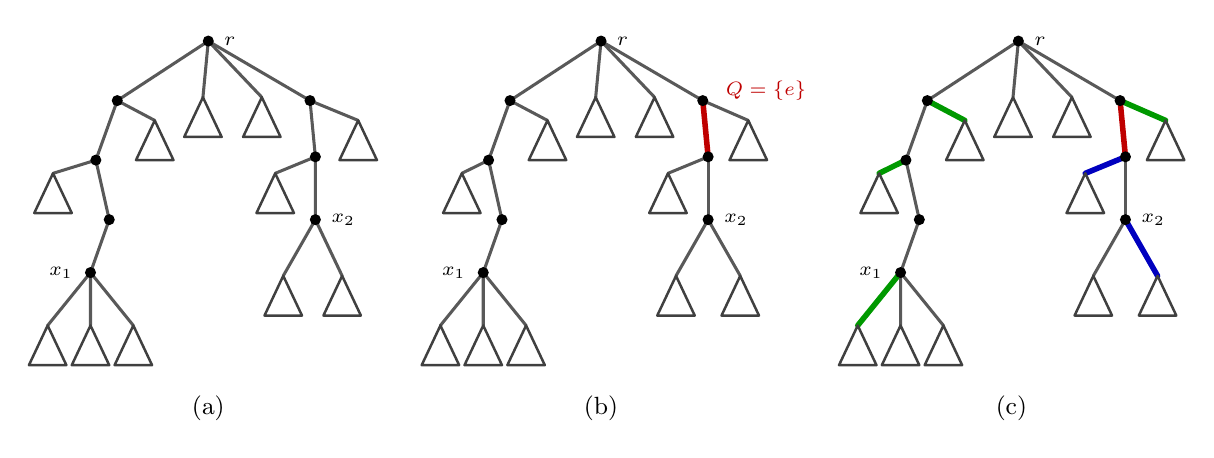
\begin{tikzpicture}[
        x=0.68cm,
        y=0.84cm,
        treeedge/.style={draw=black!65,line width=1.1pt,line cap=round},
        cutedge/.style={draw=green!60!black,line width=2pt,line cap=round},
        cutedgeblue/.style={draw=blue!75!black,line width=2pt,line cap=round},
        guessededge/.style={draw=red!75!black,line width=2pt,line cap=round},
        subtree/.style={draw=black!75,line width=0.9pt,line join=round},
    ]
        \coordinate (rOne) at (3.0,5.0);
        \coordinate (aOne) at (1.3,4.1);
        \coordinate (aTwo) at (0.9,3.2);
        \coordinate (aThree) at (1.15,2.3);
        \coordinate (xOne) at (0.8,1.5);
        \coordinate (bOne) at (4.9,4.1);
        \coordinate (bTwo) at (5.0,3.25);
        \coordinate (xTwo) at (5.0,2.3);
        \draw[treeedge] (rOne)--(aOne)--(aTwo)--(aThree)--(xOne);
        \draw[treeedge] (rOne)--(bOne)--(bTwo)--(xTwo);
        \draw[treeedge] (rOne)--(2.9,4.15) (rOne)--(4.0,4.15);
        \draw[subtree] (2.9,4.15)--(2.55,3.55)--(3.25,3.55)--cycle;
        \draw[subtree] (4.0,4.15)--(3.65,3.55)--(4.35,3.55)--cycle;
        \draw[treeedge] (aOne)--(2.0,3.8);
        \draw[subtree] (2.0,3.8)--(1.65,3.2)--(2.35,3.2)--cycle;
        \draw[treeedge] (aTwo)--(0.1,3.0);
        \draw[subtree] (0.1,3.0)--(-0.25,2.4)--(0.45,2.4)--cycle;
        \draw[treeedge] (bOne)--(5.8,3.8);
        \draw[subtree] (5.8,3.8)--(5.45,3.2)--(6.15,3.2)--cycle;
        \draw[treeedge] (bTwo)--(4.25,3.0);
        \draw[subtree] (4.25,3.0)--(3.9,2.4)--(4.6,2.4)--cycle;
        \draw[treeedge] (xOne)--(0.0,0.7) (xOne)--(0.8,0.7) (xOne)--(1.6,0.7);
        \draw[subtree] (0.0,0.7)--(-0.35,0.1)--(0.35,0.1)--cycle;
        \draw[subtree] (0.8,0.7)--(0.45,0.1)--(1.15,0.1)--cycle;
        \draw[subtree] (1.6,0.7)--(1.25,0.1)--(1.95,0.1)--cycle;
        \draw[treeedge] (xTwo)--(4.4,1.45) (xTwo)--(5.5,1.45);
        \draw[subtree] (4.4,1.45)--(4.05,0.85)--(4.75,0.85)--cycle;
        \draw[subtree] (5.5,1.45)--(5.15,0.85)--(5.85,0.85)--cycle;
        \foreach \p in {aOne,aTwo,aThree,bOne,bTwo} {\fill (\p) circle (2pt);}
        \foreach \p in {rOne,xOne,xTwo} {\fill (\p) circle (2pt);}
        \node[font=\scriptsize,anchor=west] at (3.12,5.0) {$r$};
        \node[font=\scriptsize,anchor=east] at (0.65,1.5) {$x_1$};
        \node[font=\scriptsize,anchor=west] at (5.12,2.3) {$x_2$};

        \begin{scope}[xshift=0.5cm]
        \coordinate (rTwo) at (9.6,5.0);
        \coordinate (cOne) at (7.9,4.1);
        \coordinate (cTwo) at (7.5,3.2);
        \coordinate (cThree) at (7.75,2.3);
        \coordinate (xOneTwo) at (7.4,1.5);
        \coordinate (dOne) at (11.5,4.1);
        \coordinate (dTwo) at (11.6,3.25);
        \coordinate (xTwoTwo) at (11.6,2.3);
        \draw[treeedge] (rTwo)--(cOne)--(cTwo)--(cThree)--(xOneTwo);
        \draw[treeedge] (rTwo)--(dOne);
        \draw[guessededge] (dOne)--(dTwo);
        \draw[treeedge] (dTwo)--(xTwoTwo);
        \draw[treeedge] (rTwo)--(9.5,4.15) (rTwo)--(10.6,4.15);
        \draw[subtree] (9.5,4.15)--(9.15,3.55)--(9.85,3.55)--cycle;
        \draw[subtree] (10.6,4.15)--(10.25,3.55)--(10.95,3.55)--cycle;
        \draw[treeedge] (cOne)--(8.6,3.8);
        \draw[subtree] (8.6,3.8)--(8.25,3.2)--(8.95,3.2)--cycle;
        \draw[treeedge] (cTwo)--(7.0,3.0);
        \draw[subtree] (7.0,3.0)--(6.65,2.4)--(7.35,2.4)--cycle;
        \draw[treeedge] (dOne)--(12.35,3.8);
        \draw[subtree] (12.35,3.8)--(12.0,3.2)--(12.7,3.2)--cycle;
        \draw[treeedge] (dTwo)--(10.85,3.0);
        \draw[subtree] (10.85,3.0)--(10.5,2.4)--(11.2,2.4)--cycle;
        \draw[treeedge] (xOneTwo)--(6.6,0.7) (xOneTwo)--(7.4,0.7) (xOneTwo)--(8.2,0.7);
        \draw[subtree] (6.6,0.7)--(6.25,0.1)--(6.95,0.1)--cycle;
        \draw[subtree] (7.4,0.7)--(7.05,0.1)--(7.75,0.1)--cycle;
        \draw[subtree] (8.2,0.7)--(7.85,0.1)--(8.55,0.1)--cycle;
        \draw[treeedge] (xTwoTwo)--(11.0,1.45) (xTwoTwo)--(12.2,1.45);
        \draw[subtree] (11.0,1.45)--(10.65,0.85)--(11.35,0.85)--cycle;
        \draw[subtree] (12.2,1.45)--(11.85,0.85)--(12.55,0.85)--cycle;
        \foreach \p in {cOne,cTwo,cThree,dOne,dTwo} {\fill (\p) circle (2pt);}
        \foreach \p in {rTwo,xOneTwo,xTwoTwo} {\fill (\p) circle (2pt);}
        \node[font=\scriptsize,anchor=west] at (9.72,5.0) {$r$};
        \node[font=\scriptsize,anchor=east] at (7.25,1.5) {$x_1$};
        \node[font=\scriptsize,anchor=west] at (11.72,2.3) {$x_2$};
        \node[font=\scriptsize,text=red!75!black,anchor=west] at (11.75,4.25) {$Q=\{e\}$};
        \end{scope}

        \begin{scope}[xshift=5.8cm]
        \coordinate (rThree) at (9.6,5.0);
        \coordinate (cOneThree) at (7.9,4.1);
        \coordinate (cTwoThree) at (7.5,3.2);
        \coordinate (cThreeThree) at (7.75,2.3);
        \coordinate (xOneThree) at (7.4,1.5);
        \coordinate (dOneThree) at (11.5,4.1);
        \coordinate (dTwoThree) at (11.6,3.25);
        \coordinate (xTwoThree) at (11.6,2.3);
        \draw[treeedge] (rThree)--(cOneThree)--(cTwoThree)--(cThreeThree)--(xOneThree);
        \draw[treeedge] (rThree)--(dOneThree);
        \draw[treeedge] (dOneThree)--(dTwoThree);
        \draw[guessededge] (dOneThree)--(dTwoThree);
        \draw[treeedge] (dTwoThree)--(xTwoThree);
        \draw[treeedge] (rThree)--(9.5,4.15) (rThree)--(10.6,4.15);
        \draw[subtree] (9.5,4.15)--(9.15,3.55)--(9.85,3.55)--cycle;
        \draw[subtree] (10.6,4.15)--(10.25,3.55)--(10.95,3.55)--cycle;
        \draw[treeedge] (cOneThree)--(8.6,3.8);
        \draw[cutedge] (cOneThree)--(8.6,3.8);
        \draw[subtree] (8.6,3.8)--(8.25,3.2)--(8.95,3.2)--cycle;
        \draw[treeedge] (cTwoThree)--(7.0,3.0);
        \draw[cutedge] (cTwoThree)--(7.0,3.0);
        \draw[subtree] (7.0,3.0)--(6.65,2.4)--(7.35,2.4)--cycle;
        \draw[treeedge] (dOneThree)--(12.35,3.8);
        \draw[cutedge] (dOneThree)--(12.35,3.8);
        \draw[subtree] (12.35,3.8)--(12.0,3.2)--(12.7,3.2)--cycle;
        \draw[treeedge] (dTwoThree)--(10.85,3.0);
        \draw[cutedgeblue] (dTwoThree)--(10.85,3.0);
        \draw[subtree] (10.85,3.0)--(10.5,2.4)--(11.2,2.4)--cycle;
        \draw[treeedge] (xOneThree)--(6.6,0.7);
        \draw[cutedge] (xOneThree)--(6.6,0.7);
        \draw[treeedge] (xOneThree)--(7.4,0.7) (xOneThree)--(8.2,0.7);
        \draw[subtree] (6.6,0.7)--(6.25,0.1)--(6.95,0.1)--cycle;
        \draw[subtree] (7.4,0.7)--(7.05,0.1)--(7.75,0.1)--cycle;
        \draw[subtree] (8.2,0.7)--(7.85,0.1)--(8.55,0.1)--cycle;
        \draw[treeedge] (xTwoThree)--(11.0,1.45) (xTwoThree)--(12.2,1.45);
        \draw[cutedgeblue] (xTwoThree)--(12.2,1.45);
        \draw[subtree] (11.0,1.45)--(10.65,0.85)--(11.35,0.85)--cycle;
        \draw[subtree] (12.2,1.45)--(11.85,0.85)--(12.55,0.85)--cycle;
        \foreach \p in {cOneThree,cTwoThree,cThreeThree,dOneThree,dTwoThree} {\fill (\p) circle (2pt);}
        \fill (rThree) circle (2pt);
        \fill (xOneThree) circle (2pt);
        \fill (xTwoThree) circle (2pt);
        \node[font=\scriptsize,anchor=west] at (9.72,5.0) {$r$};
        \node[font=\scriptsize,anchor=east] at (7.25,1.5) {$x_1$};
        \node[font=\scriptsize,anchor=west] at (11.72,2.3) {$x_2$};
        \end{scope}
        \node[font=\small] at (3.0,-0.55) {(a)};
        \node[font=\small,xshift=0.5cm] at (9.6,-0.55) {(b)};
        \node[font=\small] at (18.0,-0.55) {(c)};
    \end{tikzpicture}
    \caption{(a) The initial tree with centroids $r$, $x_1$ and $x_2$. (b) The guess $Q=\brc{e}$ (red dashed). (c) Green edges are cuts in the component containing $x_1$, blue edges are cuts in the component containing $x_2$, and the guessed edge $e$ remains red and dashed.}
    \label{fig:three-centroid-coverage}
    \end{figure}

        For each guess $Q$, the algorithm applies this routine to every $K\in\mathcal K_Q$ with $w\br{V_K}>B_\rho$, skips $Q$ if any full quota is infeasible, and minimizes $c(Q)+\sum_Kc_K(A_K)$. Components without vertices in $\mathcal L_H$ are left for recursion.

        \begin{algorithm}[tbp]
    \DontPrintSemicolon
    \caption{Centroid recursion with core coverage}\label{alg:centroid-max-coverage}
    \textbf{Input} Supply tree $T=(V,E,c)$, demand graph $(V,D,w)$, fixed rational parameters $0<\rho<\eta<1$\;
    \textbf{Output} An $\eta$-feasible supply-edge set $F\subseteq E$\;
    Set $B_\rho\gets\rho W$ and $B_\eta\gets\eta W$\;
    \textbf{Procedure} $\textsc{CentroidMaxCoverage}(H)$\;
    \Indp
        \If{$w\br{V_H}\leq B_\eta$}{
            \textbf{return} $\emptyset$\;
        }
        Choose a weighted centroid $r$ of $H$ for weights $\mu_H$ defined in the text. For every component $X$ of $H-r$ with $w(X)>w\br{V_H}/3$, choose a weighted centroid $x_X$ of $X$ using the restricted weights $\mu_H$, thus obtaining a set $\mathcal{L}_H$\;
        Choose a path $P_H$, such that $\mathcal{L}_H\subseteq V(P_H)$ and $|V(P_H)|\geq 3$ if $|V_H|\geq 3$. Add arbitrary unused vertices of $P_H$ to $\mathcal{L}_H$ until $|\mathcal{L}_H|=3$\;
        Let $S_H=V_H[\mathcal{L}_H]$\;
        Initialize $\cC_H\gets\emptyset$\;
        \ForEach{$Q\subseteq E(S_H)$ with $|Q|\leq2$}{
            Let $\mathcal{K}_Q=\brc{K\in H\setminus Q: V_K\cap \mathcal{L}_H\neq\emptyset}$ and let $\mathcal{K}_Q^+=\{K\in\mathcal{K}_Q:w\br{V_K}>B_\rho\}$\;
            \ForEach{$K\in\mathcal{K}_Q^+$}{
                Let $B_K=V_K[S_H]$ and set $q_K\gets w\br{V_K}-B_\rho$\;
            }
            \If{$f_K(E(K)\setminus E(B_K))\geq q_K$ for every $K\in\mathcal{K}_Q^+$}{
                \ForEach{$K\in\mathcal{K}_Q^+$}{
                    $A_K\gets\textsc{CoreQuotaCover}(f_K,c_K,q_K)$\;
                }
                Let $C_Q\gets Q\cup\bigcup_{K\in\mathcal{K}_Q^+}C_K(A_K)$ and add $C_Q$ to $\cC_H$\;
            }
        }
        Let $C_H\in\arg\min_{C\in\cC_H}\brc{c(C)}$\;
        Set $F_H\gets C_H$\;
        \ForEach{component $H'$ of $H\setminus C_H$ with $w(V_{H'})>B_\eta$}{
            $F_H\gets F_H\cup\textsc{CentroidMaxCoverage}(H')$\;
        }
        \textbf{return} $F_H$\;
    \Indm
    $F\gets\textsc{CentroidMaxCoverage}(T)$\;
    \textbf{return} $F$\;
\end{algorithm}


        \begin{theorem}\label{thm:tree-centroid-max-coverage}
            Fix rational constants $0<\rho<\eta<1$. For arbitrary integral demand weights on a supply tree, Algorithm~\ref{alg:centroid-max-coverage} runs in polynomial time and returns an $\eta$-feasible supply-edge set $F\subseteq E$ with
            \[
                c(F)\leq\Gamma_{\mathrm{MC}}(\rho,\eta)\cdot\OPTdem{T}{\rho},
            \]
            \begin{equation}\label{eq:tree-centroid-max-coverage-ratio}
                \Gamma_{\mathrm{MC}}(\rho,\eta)
                =\left\lceil\ln\left(\frac{1-\rho}{\eta-\rho}\right)\right\rceil.
            \end{equation}
        \end{theorem}
        \begin{proof}
            If $W=0$, the empty cut is feasible, so assume $W>0$. For a processed component $H$, write $h=w\br{V_H}$ and $q_H=h-B_\rho=\Phi(H)>0$, where the \emph{excess} of a component $J$ is $\Phi(J)=\max\{0,w\br{V_J}-B_\rho\}$, which is the measure of the progress of our algorithm.

            First consider the progress. Let $K\in K_Q$. If $w\br{V_K}\leq B_\eta$, its excess is zero so the component is already $\eta$-feasible. Otherwise, $q_K=w\br{V_K}-B_\rho\leq q_H$, and the cover guarantee gives
            \[
                \Phi(K\setminus U_K(A_K))
                =\max\{0,w\br{V_K}-f_K(A_K)-B_\rho\}\leq
                q_K-\br{1-1/e}\cdot q_K = q_K/e
                \leq q_H/e.
            \]
            A component $K$, such that $K\cap \mathcal L_H=\emptyset$, is contained in a component of $H\setminus\mathcal L_H$, so its demand is at most $w\br{V_H}/3$ and its excess is at most
            \[
                \Phi(K\setminus U_K(A_K))
                \leq\max\{0,w\br{V_H}/3-B_\rho\}\leq w\br{V_H}/3-B_\rho\leq w\br{V_H}/3-B_\rho/3 = q_H/3<q_H/e,
            \]
            since $e<3$. Thus every child has excess at most $1/e$ times its parent's. Initially $\Phi(T)=(1-\rho)\cdot W$. After
            \[
                L=\left\lceil\ln\left(\frac{1-\rho}{\eta-\rho}\right)\right\rceil
            \]
            generations, every component $J$ has excess at most 
            \[
            \Phi(J)\leq \frac{\Phi(T)}{e^L}=\frac{(1-\rho)\cdot W}{e^L}\leq (\eta-\rho)\cdot W=B_\eta-B_\rho.
            \]
            Therefore, $w\br{J}\leq B_\eta$. Thus the output is $\eta$-feasible and the recursion has at most $L$ levels.

            Next bound the cost of one processed component. Let $F_H^*$ be an optimal $B_\rho$-feasible edge set and take the matching guess $Q^*\subseteq F_H^*\cap E(S_H)$ described above. For each $K\in\mathcal K_{Q^*}$, all vertices in $\mathcal L_H$ lie in one component of $H\setminus F_H^*$. Therefore $F_H^*\cap E(K)$ has no edge on $B_K$, and the component containing $B_K$ after this restriction is contained in an optimal component. Thus $\OPT_{MC,B_K}\br{K}\leq c(F_H^*\cap E(K))$. The score of this feasible guess is at most
            \[
                c(Q^*)+\sum_K\OPT_{MC,B_K}\br{K}
                \leq c(F_H^*)
                =\OPT_{B_\rho}(H).
            \]
            Since the algorithm chooses a least-cost guess and each actual core-boundary edge set has cost at most that of its corresponding proposed set, its local edge set $C_H$ satisfies $c(C_H)\leq\OPT_{B_\rho}(H)$.

            Let $F_H$ be all edges returned below $H$, and let $d(H)$ be the maximum number of nonterminal calls on a path in this recursion subtree. Using induction in a manner similar to previous proofs, we obtain
            \begin{equation}\label{eq:tree-centroid-recursive-cost}
                c(F_H)\leq d(H)\cdot \OPT_{B_\rho}(H).
            \end{equation}
            It is immediate for terminal components. For a nonterminal component of depth $d$, let $H_1,\ldots,H_m$ be its children. By induction and the one-call bound,
            \[
                c(F_H)\leq\OPT_{B_\rho}(H)
                +(d-1)\cdot \sum_{i=1}^m\OPT_{B_\rho}(H_i).
            \]
            Restricting an optimal $B_\rho$-feasible cut of $H$ to the pairwise edge-disjoint children gives \[
            \sum_i\OPT_{B_\rho}(H_i)\leq\OPT_{B_\rho}(H),
            \] 
            proving~\eqref{eq:tree-centroid-recursive-cost}. Since $d(T)\leq L$ and $\OPT_{B_\rho}(T)=\OPTdem{T}{\rho}$, this completes the proof.
        \end{proof}

        \subsection{A Hybrid LP-Separator Recursion Approach}

Assume $0<\rho<\eta<3\rho<1$, and put
\[
    \delta=\eta-\rho,
    \qquad
    x=\ln\left(\frac{2\rho}{\delta}\right),
    \qquad
    k=\left\lfloor x\right\rfloor.
\]
The hybrid first applies anchored-LP rounding with target $\tau=\rho+e^k\delta$, then runs separator recursion on the resulting components. Since $e^k\delta\leq2\rho$, the LP target satisfies $\tau\leq3\rho<1$, and at most $k$ separator rounds suffice.

\subsubsection{The hybrid procedure}
\begin{algorithm}[tbp]
    \DontPrintSemicolon
    \caption{Hybrid LP-separator recursion}\label{alg:hybrid-lp-centroid}
    \textbf{Input} Supply tree $T=(V,E,c)$, demand graph $(V,D,w)$, and fixed rational parameters $0<\rho<\eta<3\rho<1$\;
    \textbf{Output} An $\eta$-feasible supply-edge set $F\subseteq E$\;
    \If{$W=0$}{
        \textbf{return} $F=\emptyset$\;
    }
    Set $\delta\gets\eta-\rho$, $x\gets\ln(2\rho/\delta)$, and $k\gets\lfloor x\rfloor$\;
    Set $\tau\gets\rho+e^k\delta$\;
    Run the anchored-LP algorithm with feasibility target $\tau$. Let $F_0$ be the returned cut and let $\cH_0$ be the components of $T\setminus F_0$\;
    Set $B_\rho\gets\rho W$, $B_\eta\gets\eta W$, and $F\gets F_0$\;
    \ForEach{$H\in\cH_0$ with $w\br{V_H}>B_\eta$}{
        Set $\rho_H\gets B_\rho/w\br{V_H}$ and $\eta_H\gets B_\eta/w\br{V_H}$\;
        Run Algorithm~\ref{alg:centroid-max-coverage} on the instance induced by $V_H$ with parameters $\rho_H,\eta_H$, obtaining a supply-edge set $F_H$\;
        $F\gets F\cup F_H$\;
    }
    \textbf{return} $F$\;
\end{algorithm}

Apply Corollary~\ref{cor:tree-general-demand-bicriteria} with feasibility target $\tau=\rho+e^k\delta$, and let $F_0$ be the resulting supply-edge set and $\cH_0$ the components of $T\setminus F_0$. Every $H\in\cH_0$ has demand at most $\tau W$, and the normalization cost satisfies
\begin{equation}\label{eq:tree-hybrid-normalization-cost}
    c\br{F_0}
    \leq
    \left(2+\frac{2\rho}{e^k\delta}\right)\cdot\OPT_{B_\rho}(T).
\end{equation}

For each $H\in\cH_0$ with $w\br{V_H}>B_\eta$, run Algorithm~\ref{alg:centroid-max-coverage} on the instance induced by $V_H$ with local parameters
\[
    \rho_H=\frac{B_\rho}{w\br{V_H}},
    \qquad
    \eta_H=\frac{B_\eta}{w\br{V_H}}.
\]
These parameters make the algorithm's local budgets equal to $B_\rho$ and $B_\eta$, respectively. Let $F_H$ be its returned supply-edge set, and set $F=F_0\cup\bigcup_{H\in\cH_0}F_H$.

\begin{theorem}\label{thm:tree-hybrid-recursion}
    Fix rational parameters $0<\rho<\eta<3\rho<1$. For integral demand weights on a supply tree, the hybrid algorithm returns an $\eta$-feasible supply-edge set $F$ satisfying
    \[
        c\br{F}\leq\Gamma_{\mathrm{H}}(\rho,\eta)\cdot\OPTdem{T}{\rho},
    \]
    where
    \begin{equation}\label{eq:tree-hybrid-ratio}
        \Gamma_{\mathrm{H}}(\rho,\eta)
        =e+1+\ln\left(\frac{2\rho}{\eta-\rho}\right).
    \end{equation}
    For fixed $\rho$ and $\eta$, the algorithm runs in polynomial time.
\end{theorem}
\begin{proof}
    Let $\delta=\eta-\rho$, $x=\ln(2\rho/\delta)$, $k=\lfloor x\rfloor$, and $s=x-k\in[0,1)$. Since $k\leq x$, we have $e^k\delta\leq2\rho$ and hence $\tau=\rho+e^k\delta\leq3\rho<1$. By Corollary~\ref{cor:tree-general-demand-bicriteria}, the normalization cut satisfies~\eqref{eq:tree-hybrid-normalization-cost}.

    By the LP normalization, $w\br{V_H}\leq\tau W=(\rho+e^k\delta)W$, so every normalized component's excess above $B_\rho$ is at most $e^k\delta W$. Each separator-coverage round reduces the excess of every child by a factor of at least $e$. Hence after at most $k$ rounds all components have excess at most $\delta W=B_\eta-B_\rho$ and are $\eta$-feasible. At each depth, the processed components are pairwise edge-disjoint, and restricting an optimal $B_\rho$-feasible cut of $T$ to them shows that the total cost charged at that depth is at most $\OPT_{B_\rho}(T)$. The separator recursion therefore adds cost at most $k\OPT_{B_\rho}(T)$.

    Combining this with~\eqref{eq:tree-hybrid-normalization-cost} gives
    \[
        c\br{F}\leq
        \left(k+2+\frac{2\rho}{e^k\delta}\right)\OPT_{B_\rho}(T).
    \]
    Since $x=k+s$ and $e^k\delta=2\rho/e^s$, the coefficient is
    \[
        k+2+\frac{2\rho}{e^k\delta}
        =k+2+e^s
        =x+2+e^s-s
        \leq x+e+1,
    \]
    where $e^s-s\leq e-1$ for $0\leq s<1$. This proves the claimed bound. Since all of the constants in this construction ultimately depend only on the fixed parameters $\rho$ and $\eta$, the algorithm runs in polynomial time.
\end{proof}

        \subsubsection{Combined guarantee}


        The anchored LP and centroid maximum-coverage algorithms apply for all $0<\rho<\eta<1$, while the hybrid algorithm also applies when $0<\rho<\eta<3\rho<1$. Taking the best applicable guarantee gives the following result.

        \begin{corollary}\label{cor:tree-best-bicriteria}
            For every fixed rational $0<\rho<\eta<1$, \textsc{Graph Partitioning with Demands} on supply trees admits a polynomial-time algorithm which returns an $\eta$-feasible solution of cost at most $
                \Gamma_{\mathrm{tree}}(\rho,\eta)\cdot \OPTdem{T}{\rho}$,
            where
            \[
                \Gamma_{\mathrm{tree}}(\rho,\eta)
                =
                \begin{cases}
                    \displaystyle
                    \min\left\{
                        \Gamma_{\mathrm{LP}}(\rho,\eta),
                        \Gamma_{\mathrm{H}}(\rho,\eta),
                        \Gamma_{\mathrm{MC}}(\rho,\eta)
                    \right\},
                        &0<\rho<\eta<3\rho<1,\\[2mm]
                    \displaystyle
                    \min\left\{
                        \Gamma_{\mathrm{LP}}(\rho,\eta),
                        \Gamma_{\mathrm{MC}}(\rho,\eta)
                    \right\},
                        &\text{otherwise},
                \end{cases}
            \]
            where:
                \begin{itemize}
                \item $\Gamma_{\mathrm{LP}}(\rho,\eta)=\frac{2\eta}{\eta-\rho}$,
                \item $\Gamma_{\mathrm{H}}(\rho,\eta)=e+1+\ln\left(\frac{2\rho}{\eta-\rho}\right)$ for $0<\rho<\eta<3\rho<1$,
                \item $\Gamma_{\mathrm{MC}}(\rho,\eta)
                =\left\lceil\ln\left(\frac{1-\rho}{\eta-\rho}\right)\right\rceil$.
                \end{itemize}
        \end{corollary}

        
        Figures~\ref{fig:tree-approximation-ratio} and~\ref{fig:tree-approximation-ratio-3d} illustrate the combined tree approximation guarantee $\Gamma_{\mathrm{tree}}(\rho,\eta)$ over the relevant ranges of $\rho$ and $\eta$. We observe, that for almost all choices of parameters our approximation ratios are relatively close to $1$ and usually are below $4$. Only for choices of $\eta$ very close to $\rho$ the approximation ratios start to increase significantly.
        \begin{figure}[!tbp]
  \centering
  % The standalone PGFPlots output is cached so manuscript builds only include
  % the PDF. Rebuild it from figures/tree_approximation_ratio_2d_plot.tex when
  % the diagram itself changes.
  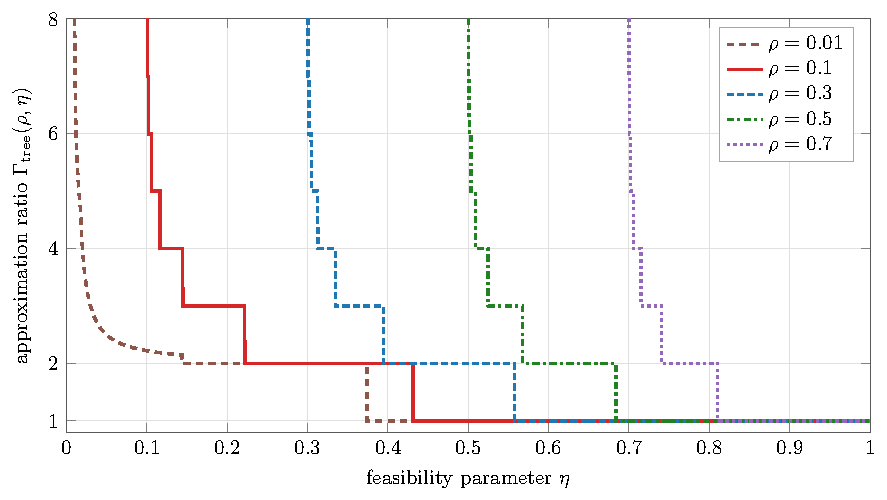
\includegraphics[width=0.92\textwidth]{figures/generated/tree_approximation_ratio_2d_plot.pdf}
  \caption{The combined approximation ratio from Corollary~\ref{cor:tree-best-bicriteria} as a function of $\eta$ for representative values of $\rho$. Values above $8$ are capped at $8$.}
  \label{fig:tree-approximation-ratio}
\end{figure}

        \begin{figure}[!tbp]
  \centering
  % Rendered on demand from tree_approximation_ratio_3d_plot.tex.
  % Keeping the dense PGFPlots surface as a PDF avoids rebuilding it with
  % every manuscript compilation.
  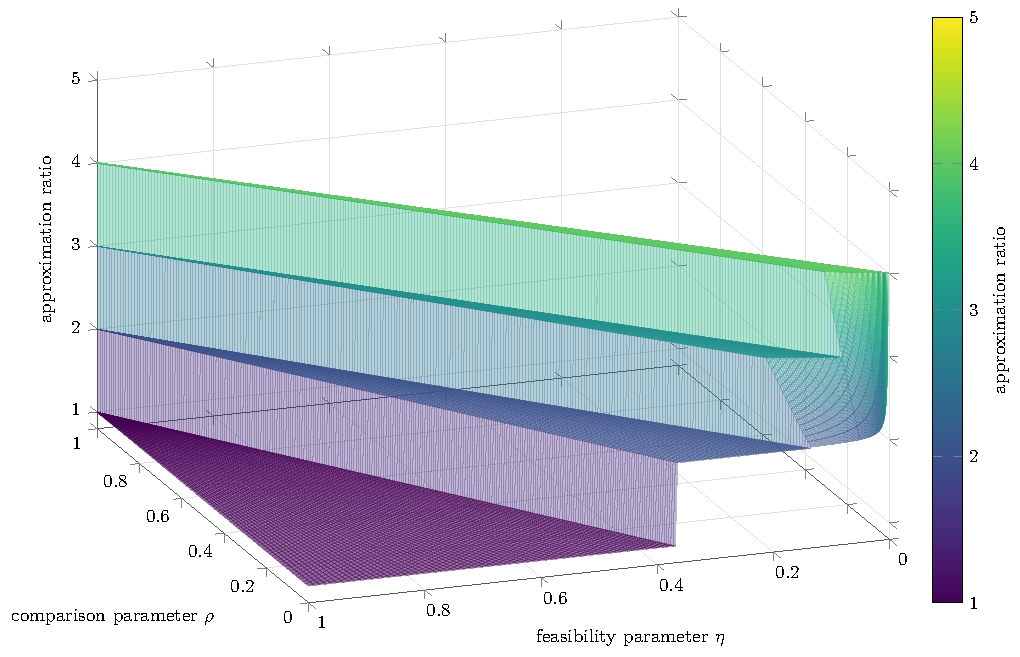
\includegraphics[width=0.94\textwidth]{figures/generated/tree_approximation_ratio_3d_plot.pdf}
  \caption{Combined tree approximation guarantee $\Gamma_{\mathrm{tree}}(\rho,\eta)$ from Corollary~\ref{cor:tree-best-bicriteria}, over $0<\rho<\eta<1$ (shown for $0.005\leq\rho\leq0.995$). Below the threshold, the height is the minimum of the anchored-LP, recursive, and hybrid bounds; above it, the direct dynamic program gives ratio $1$. Heights are capped at $12$. The plateaus reflect floor-log terms in the recursive and hybrid bounds.}
  \label{fig:tree-approximation-ratio-3d}
\end{figure}


        \subsection{Consequences for hierarchical clustering on trees}

        Combining Theorem~\ref{thm:tree-centroid-max-coverage} with Theorem~\ref{thm:hc-gpd-transfer} gives a $\frac{4e}{e-1}$-approximation for \textsc{Hierarchical Clustering with Demands} on trees.

        \begin{corollary}\label{cor:tree-hc-improved}
            There is a polynomial-time $\frac{4e}{e-1}$-approximation algorithm for \textsc{Hierarchical Clustering with Demands} on supply trees.
        \end{corollary}
        \begin{proof}
            Set $\rho=\frac12$ and $\eta=\frac{e+1}{2e}$. Then
            \[
                \frac{1-\rho}{\eta-\rho}=e,
                \qquad
                \Gamma_{\mathrm{MC}}(\rho,\eta)=\left\lceil\ln e\right\rceil=1.
            \]
            Theorem~\ref{thm:tree-centroid-max-coverage} therefore gives a polynomial-time subroutine with $\gamma(\eta)=1$. By Theorem~\ref{thm:hc-gpd-transfer}, the resulting approximation ratio is
            \[
                \frac{2}{1-\eta}=\frac{4e}{e-1}.
            \]
        \end{proof}

